\begin{figure}[t!]
    \centering
    \begin{subfigure}[t]{0.5\columnwidth}
        \centering
        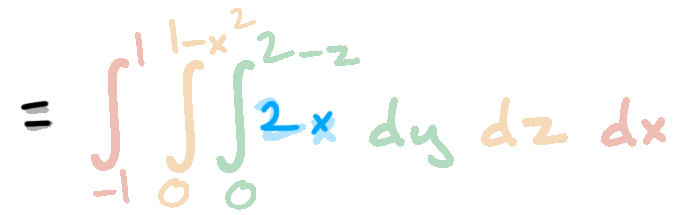
\includegraphics[width=1\columnwidth]{figures/slowink_presenter}
        \caption{Lorem ipsum}
    \end{subfigure}%
    ~ 
    \begin{subfigure}[t]{0.5\columnwidth}
        \centering
        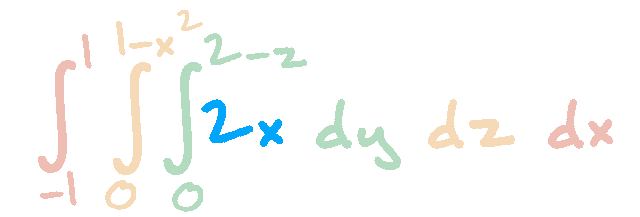
\includegraphics[width=1\columnwidth]{figures/slowink_audience}
        \caption{Lorem ipsum}
    \end{subfigure}
            ~
      \begin{subfigure}[t]{0.5\columnwidth}
        \centering
        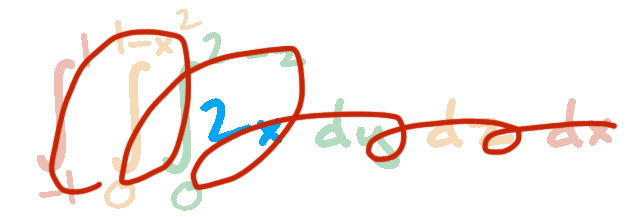
\includegraphics[width=1\columnwidth]{figures/fastink_presenter}
        \caption{Lorem ipsum}
    \end{subfigure}%
    ~ 
    \begin{subfigure}[t]{0.5\columnwidth}
        \centering
        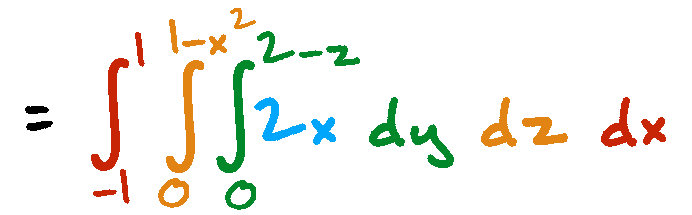
\includegraphics[width=1\columnwidth]{figures/fastink_audience}
        \caption{Lorem ipsum}
    \end{subfigure}
    \caption{Inking to reveal}
\end{figure}

\begin{figure}[t!]
    \centering
    \begin{subfigure}[t]{0.5\columnwidth}
        \centering
        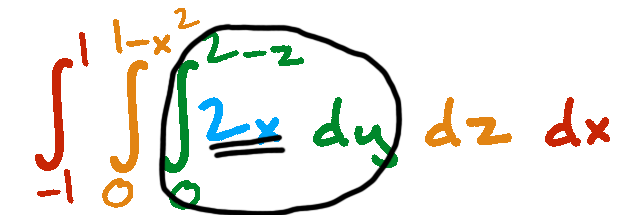
\includegraphics[width=1\columnwidth]{figures/annotate_presenter}
        \caption{Lorem ipsum}
    \end{subfigure}%
    ~ 
    \begin{subfigure}[t]{0.5\columnwidth}
        \centering
        \includegraphics[width=1\columnwidth]{figures/annotate_audience}
        \caption{Lorem ipsum}
    \end{subfigure}
      
    \caption{Inking to annotate}
\end{figure}

\section{Aparecium}

Based on these design goals, we developed \interface, a presentation system that combines electronic slides with inking interactions. 

With \interface, presenters pre-author slides to organize and refine the visual aesthetics of their material.
%
Unlike traditional electronic slides, presenters do not specify beforehand when, how, or in which order the visual elements in the slide will appear via scripted animation effects. Instead, they simply specify which elements will be displayed to the audience immediately versus which elements will be revealed in real time. 

The key innovation of \interface\ is in how presenters deliver the pre-authored content.  The main mode of interaction at presentation time is inking, but instead of just adding strokes to the slide, inking supports three functions depending on the context: it can (1) reveal pre-authored slide elements to the audience, (2) add ink strokes on top of the slide, or (3) adjust the slide layout by creating blank space. Inking allows presenters to have flexibility and fine-grained control over when, how much, and how fast to reveal elements on the slide.
%
At the same time, the ability to reveal pre-authored content allows presenters to not worry about writing or drawing neatly.
%
Presenters can also add extra writing or annotations on top of pre-authored elements, and create blank space if necessary. 
%
All of these interactions are implemented as modeless pen interactions.

Here we elaborate on slide authoring and inking in our system.
%\begin{figure*}
%  \centering
%  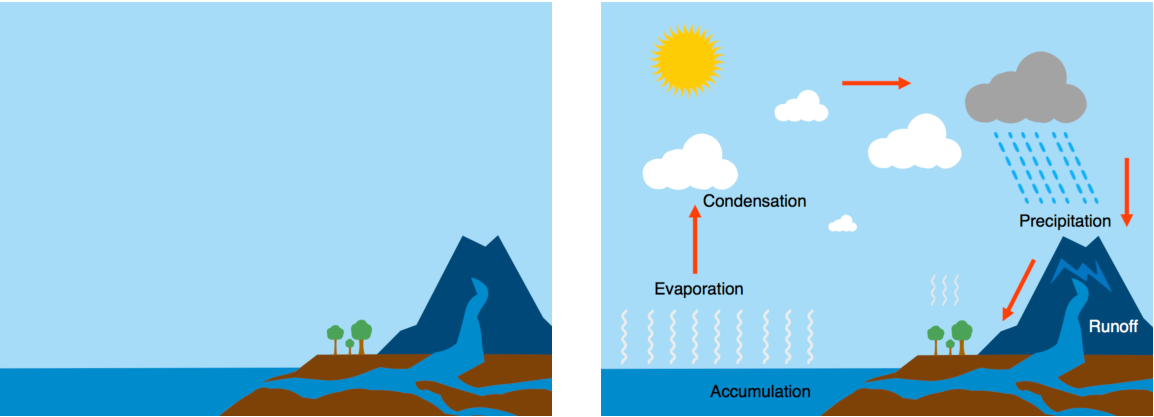
\includegraphics[width=2.0\columnwidth]{figures/watercycle}
%  \caption{}~\label{fig:watercycle}
%\end{figure*}

\begin{figure}[t!]
    \centering
    \begin{subfigure}[t]{0.48\columnwidth}
        \centering
        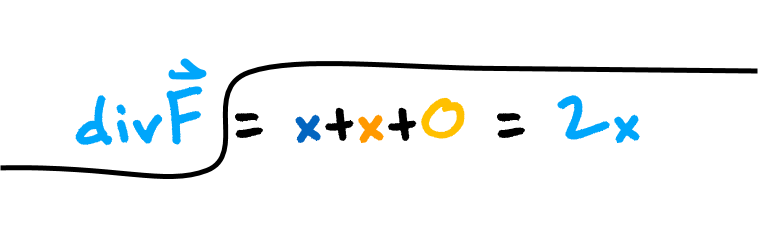
\includegraphics[width=1\columnwidth]{figures/create_space1}
        \caption{Lorem ipsum}
    \end{subfigure}%
    ~ 
    \begin{subfigure}[t]{0.48\columnwidth}
        \centering
        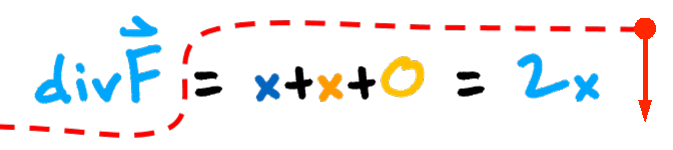
\includegraphics[width=1\columnwidth]{figures/create_space2}
        \caption{Lorem ipsum}
    \end{subfigure}
    ~
        \begin{subfigure}[t]{1\columnwidth}
        \centering
        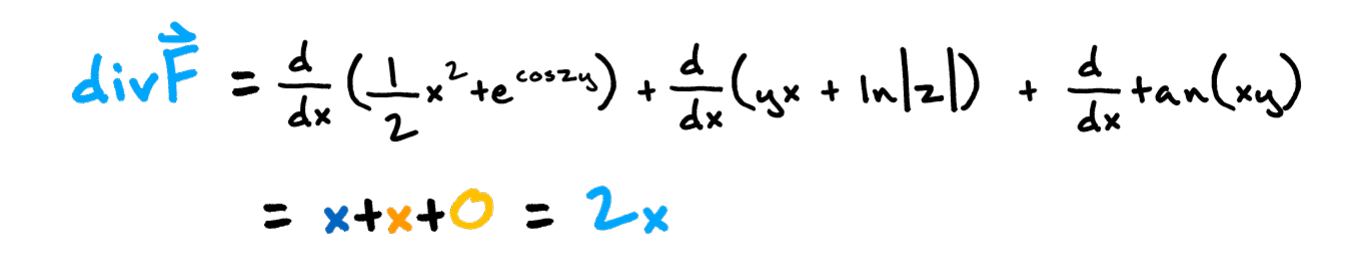
\includegraphics[width=1\columnwidth]{figures/create_space3}
        \caption{Lorem ipsum}
    \end{subfigure}  
    \caption{Creating space}
\end{figure}



\subsection{Slide authoring}
Slides in \interface\ can be authored using any existing slide presentation software (e.g., PowerPoint, Keynote, GoogleSlides). They can include typed text or images, as well as, hand drawn ink strokes. Instead of specifying animation effects on these slide elements, presenters separate them into two layers for each slide. The background layer is always visible and it is what the audience sees initially. The foreground layer is initially only visible on the presenter view, but presenters can reveal parts of it to the audience during delivery. Presenters also have the option of preparing a third layer, the notes layer, which is only visible on the presenter view and acts as transparent speaker notes placed on top of the slides. Layers in \interface\ are represented as bitmap images. (Figure~\ref{fig:watercycle})

\begin{figure*}[ht!]
    \centering
    \begin{subfigure}[t]{0.32\textwidth}
        \centering
        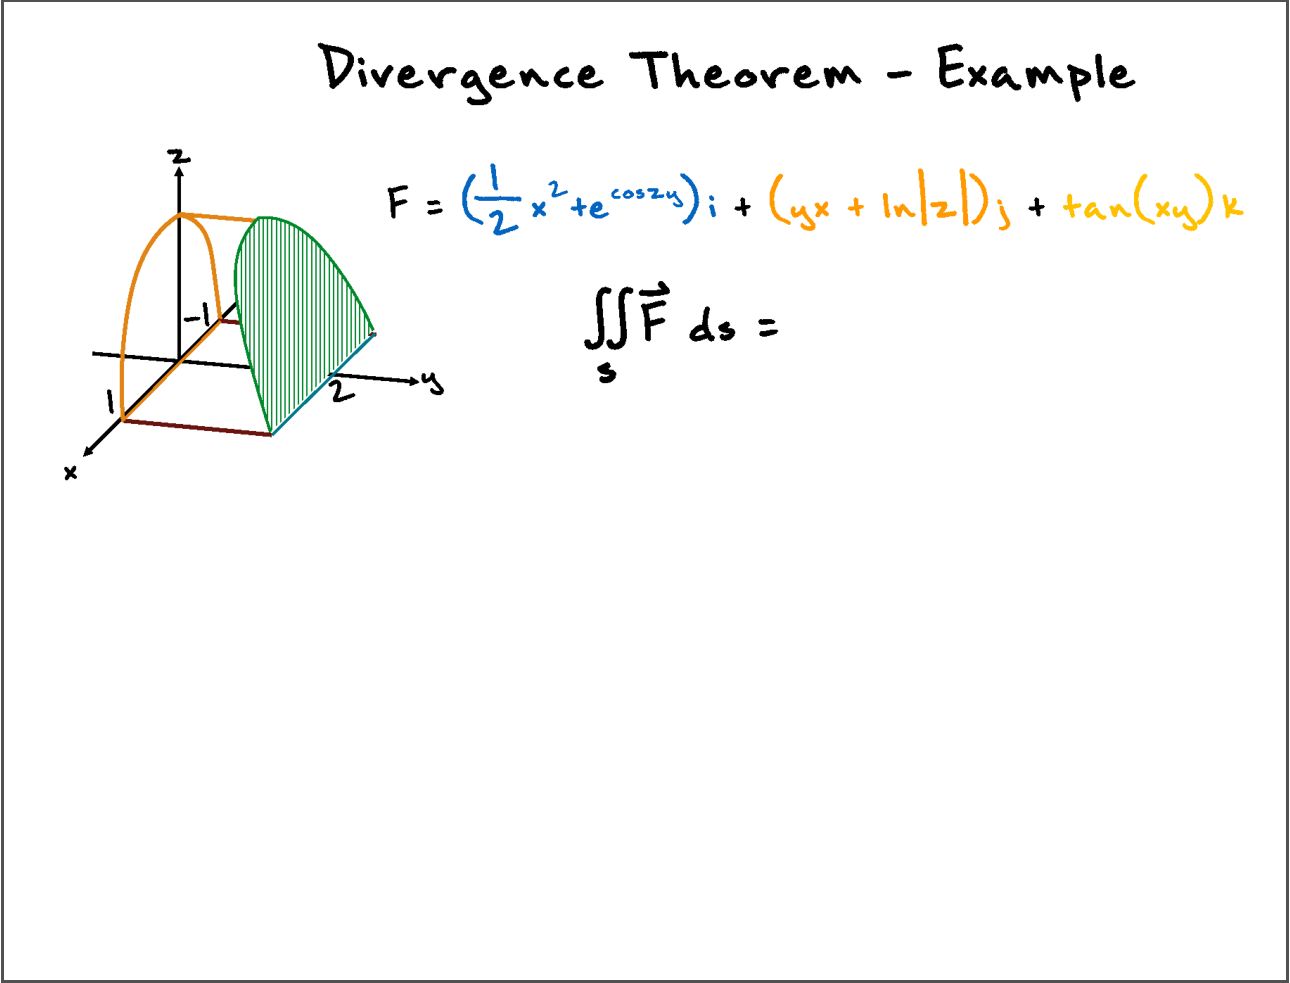
\includegraphics[width=1\columnwidth]{figures/videoslide1}
        \caption{Lorem ipsum}
    \end{subfigure}%
    ~ 
    \begin{subfigure}[t]{0.32\textwidth}
        \centering
        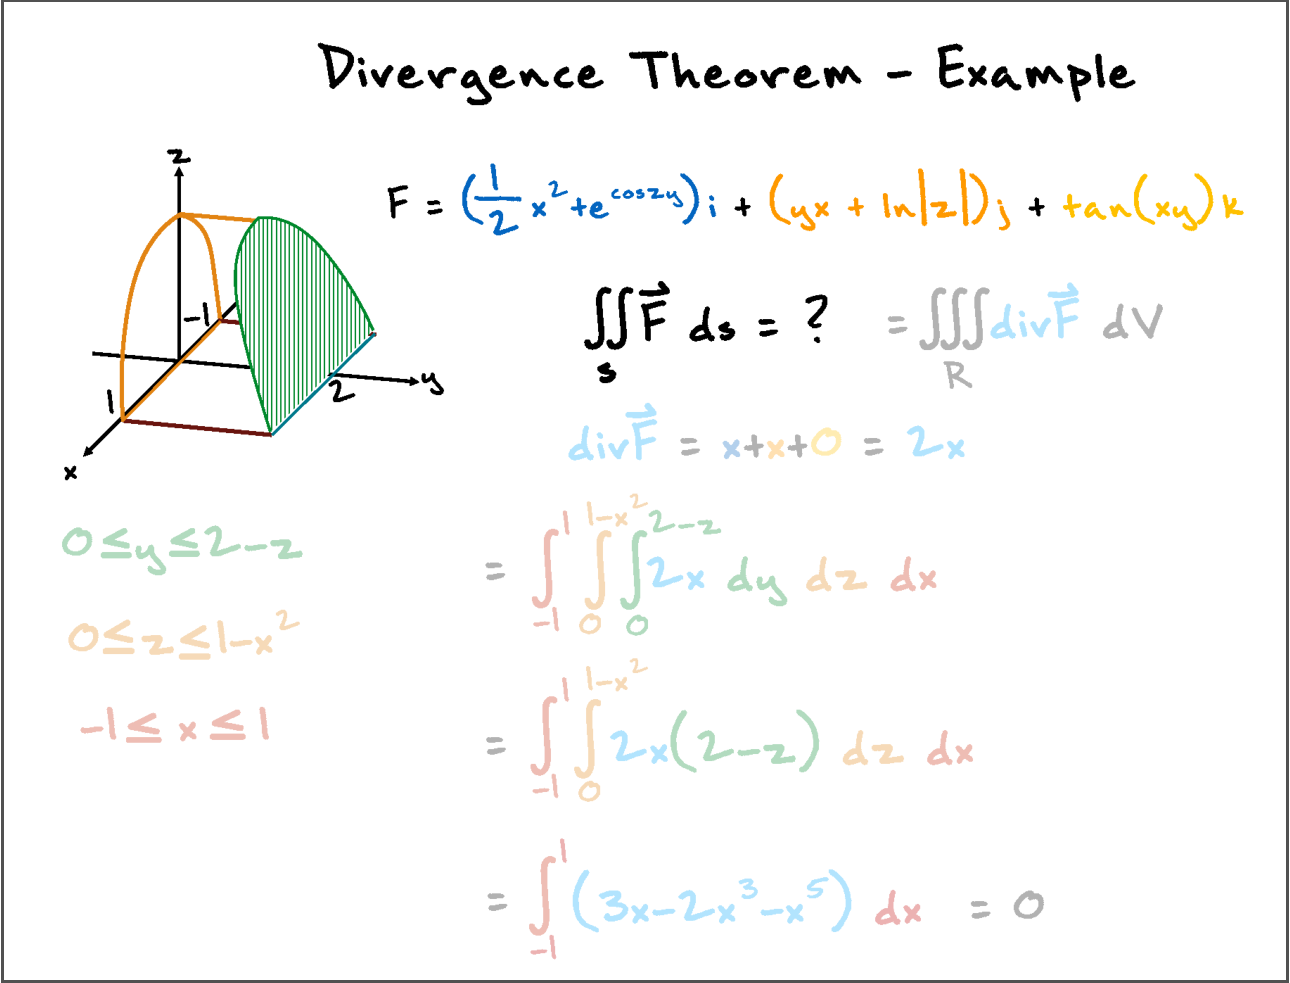
\includegraphics[width=1\columnwidth]{figures/videoslide2}
        \caption{Lorem ipsum}
    \end{subfigure}
    ~
        \begin{subfigure}[t]{0.32\textwidth}
        \centering
        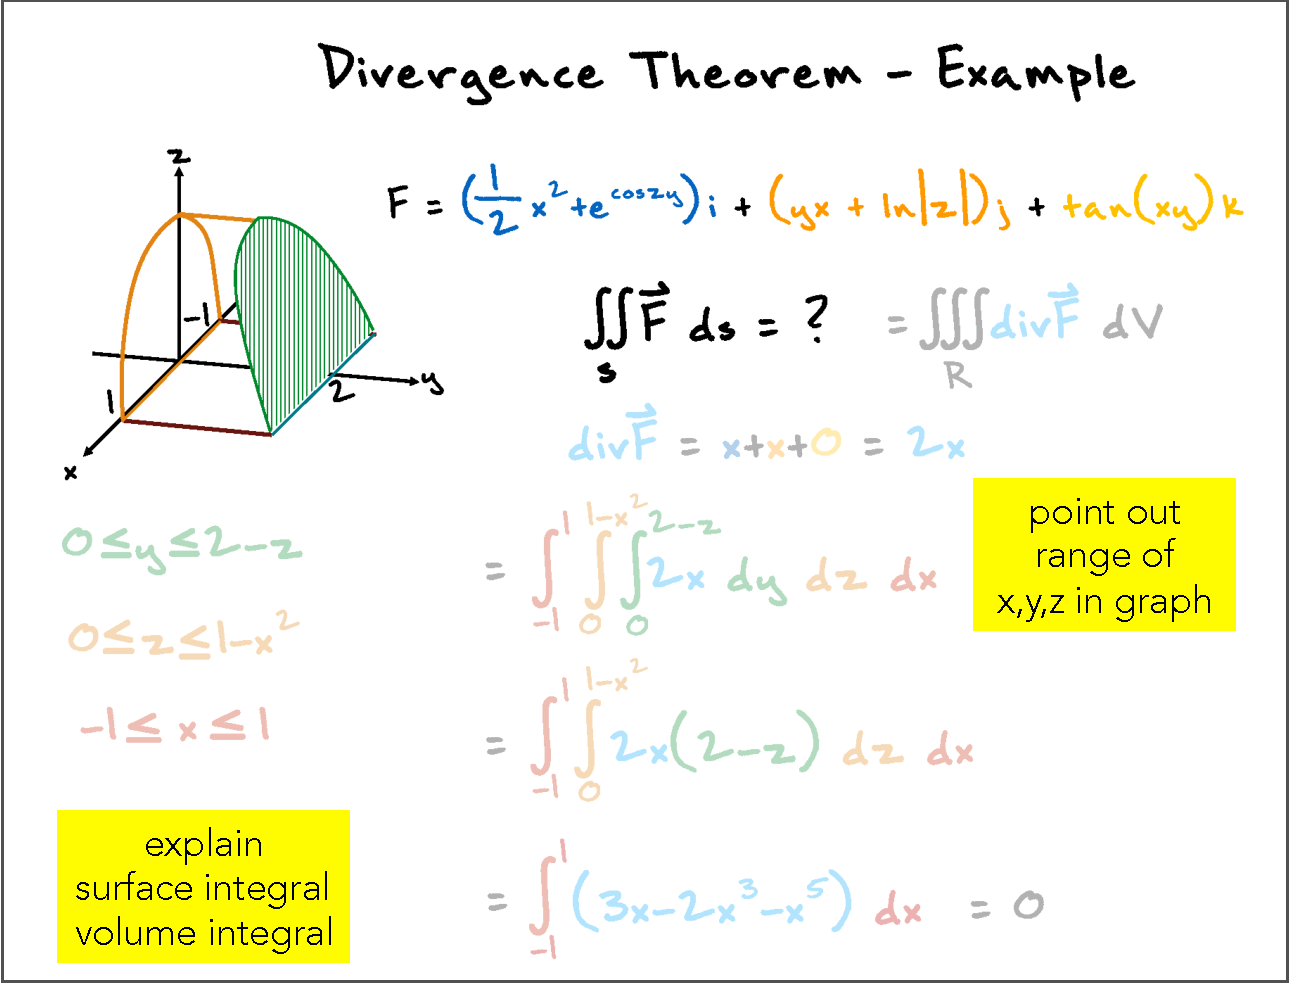
\includegraphics[width=1\columnwidth]{figures/videoslide3}
        \caption{Lorem ipsum}
    \end{subfigure}
    \caption{Slide Layers}
\end{figure*}

\subsection{Inking during delivery}
%

\interface\ enables robust, modeless inking operations at presentation time by leveraging the structure of the pre-authored slide content. Each of the three inking functions uses this structure in different ways. 

\subsubsection{Reveal}
To reveal content to the audience, the presenter inks over the relevant portion of the foreground layer.
%
At the end of each stroke, the system computes a subset of the surrounding foreground pixels to display. 
%
For each point, $s_i$ on the stroke, the closest foreground pixel, $p_i$ is computed. If the distance between $p_i$ and $s_i$ is within a threshold $\alpha$, a flood-fill is performed starting from $p_i$ to neighboring foreground pixels. The value of $\alpha$ determines how precisely the user has to ink in order to reveal the underlying content. \wil{Maybe say something about how we set $\alpha$?}
%
The extent of the flood-fill is limited by two additional thresholds $\beta$ and $\gamma$ on (1) the distance from $p_i$, and (2) the color difference (\wil{What color space?}) from $p_i$. 
%
To give presenters finer-grained control over the extent of the reveal, $\beta$ and $\gamma$ vary according to the velocity of the presenter's ink stroke. \wil{We should probably add the formula.} 

Our algorithm has several important properties. Bounding the flood-fill with $\beta$ and $\gamma$ ensures that the revealed content is localized around the user stroke and prevents ``bleeding'' across regions with very different colors. For example (\wil{add example}). 
%
In addition, modulating $\beta$ and $\gamma$ based on the stroke velocity allows presenters to reveal with different levels of precision. 
%
To show a small piece of content, the presenter can ink slowly over the relevant foreground region. This interaction is useful when the presenter wants to simulate writing in real-time, or needs to reveal a specific element in a dense slide (e.g., just the numerator in a fraction). \wil{Add figure or reference video?}
%
In other situations, users may want to reveal larger pieces of content more efficiently. For example, in \wil{Figure X}, the presenter reveals all of \wil{X} at once to save time before focusing on \wil{Y}. In this case, users can ink quickly and roughly (e.g., by scribbling) over a foreground region.
\wil{Here, we can maybe use the map example with arrows and say that if the presenter is running short on time, they can quickly scribble to reveal all the north america arrows and then spend more time focusing on individual arrows in other parts of the world.}


\if 0
If the presenter inks slowly, only a small neighborhood close to the original stroke is revealed. This is useful when the presenter wants to simulate writing in real-time, and reveal, for example, a part of a character or a diagram.
%
If the presenter inks quickly (e.g., scribbles), a larger neighborhood is revealed. This allows presenters, for instance, to swiftly reveal an entire image or a line of text without having to ink over them precisely.  \val{Figure showing user tracing over a formula, one character at a time.} \wil{I think it would be nice to motivate slow and fast inking with more specific examples that we describe in more detail and show in the form of figures and/or in the video. For slow inking, maybe we can describe an example with a formula where the presenter introduces terms one at a time. For fast inking, we can maybe use the map example with arrows and say that if the presenter is running short on time, they can quickly scribble to reveal all the north america arrows and then spend more time focusing on individual arrows in other parts of the world.}
\fi

\subsubsection{Annotate}
Presenters sometimes add new (i.e., unauthored) information to a slide on-the-fly during a presentation.
%
For example, a lecturer may circle an important concept for emphasis or explicitly label part of a diagram. \val{They can add full line}
%
To make such annotations in /interface, the presenter simply inks over empty (or already revealed) pixels on the foreground layer. If less than \wil{X\%} of the pixels in the user stroke are within the $\alpha$ threshold of an unrevealed foreground pixel, the system treats the stroke as an annotation. To ensure that the annotation stands out from the surrounding slide content, \interface\ computes the average color of the slide around the stroke and sets the ink to a complementary color. \val{Figure of annotation over revealed element and annotation on empty background}. 

\subsubsection{Create Space}
In some cases, presenters may want extra space to insert new content in a slide, for example, to add an item to an existing list, a word in a sentence, or an extra line of explanation. These situations can arise as a result of a mistake in the preparation phase (e.g., the presenter forgets to list an item), as well as from presenter-audience interaction (e.g., the audience requests extra explanation). \interface\ allows presenters to create empty space from ink strokes. First, the presenter draws a curve where the empty space should be created. At the end of the curve, if the presenter holds down the pen for more than 0.5 seconds, the curve turns into a red dashed stroke, indicating that the presenter can start expanding the space around the curve. As the presenter moves the pen along one of the axis-aligned directions, empty space is created and expanded from the curve in that direction.  As the space grows, the foreground content shifts accordingly. \val{Figure showing the steps.}
